\RequirePackage[l2tabu,orthodox]{nag}
\documentclass[bachelors,a4paper,gu]{chalmers-thesis}
\usepackage[firstinits=true,style=alphabetic,backend=biber]{biblatex}
\usepackage[swedish,english]{babel}
\usepackage[utf8]{inputenc}
\usepackage{amsfonts,amsmath,amsthm}
\usepackage{caption}
\usepackage{color}
\usepackage{csquotes}
\usepackage{hyperref}
\usepackage{listings}
\usepackage{mathtools}
\usepackage{microtype}
\usepackage{subfig}
\usepackage{subfiles}
\usepackage{tikz}
\usepackage{url}
\usepackage{verbatim}

\title{Formalisering av Algoritmer och Matematiska Bevis}
\subtitle{And stuff...}
\author{Jesper Andersson\and Daniel Oom\and Niclas Ståhl\and Åsa Lideström\and Anders Sjöberg}
\thesisin{Computer Science}
\department{Department of Stuff}
\division{Divsion...?}
\reportno{2013:11}
\copyrightyear{2013}

\coverfigure{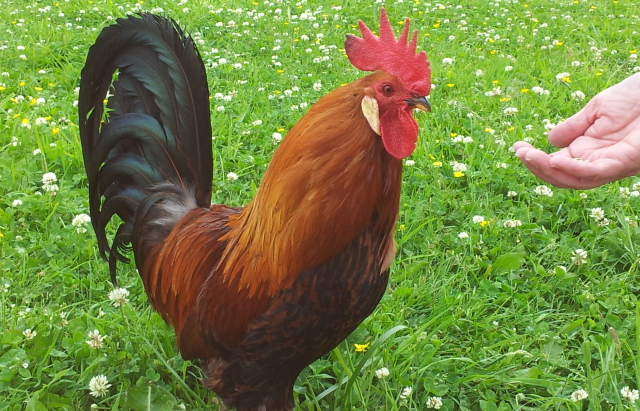
\includegraphics[width=\textwidth,height=\paperheight,keepaspectratio]{figures/Tupp}}
\covercaption{Some explanation}

\firstabstract{Apa}
\keywords{Some stuff, More stuff, Stuff}

\preface{Apa}
\acknowledgements{Apa}

\extrafrontmatter{\presectiontitle{Nomenclature} Test}

\DeclareFieldFormat[article]{title}{#1}
\DeclareFieldFormat[article]{volume}{\mkbibbold{#1}}
\renewbibmacro{in:}{}
\DeclareFieldFormat[article]{pages}{#1}
\renewbibmacro*{journal+issuetitle}{
  \usebibmacro{shortjournal}
  \setunit*{\addspace}
  \iffieldundef{series}{}{\newunit\printfield{series}\setunit{\addspace}}
  \usebibmacro{volume+number+eid}
  \setunit{\addspace}
  \usebibmacro{issue+date}
  \setunit{\addcolon\space}
  \usebibmacro{issue}
  \newunit}

\addbibresource{report.bib}

%\pagestyle{fancy}
%\lhead{Formalisering av Algoritmer och Matematiska Bevis}
%\rhead{Grupp 11}

\newcommand{\coq}{{\sc Coq}}
\newcommand{\ssr}{{\sc SSReflect}}
\newcommand{\C}[1]{\mbox{\lstinline`#1`}}
\let\L=\lstinline

\definecolor{dkblue}{rgb}{0,0.1,0.5}
\definecolor{lightblue}{rgb}{0,0.5,0.5}
\definecolor{dkgreen}{rgb}{0,0.4,0}
\definecolor{dk2green}{rgb}{0.4,0,0}
\definecolor{dkviolet}{rgb}{0.6,0,0.8}
\definecolor{shadethmcolor}{rgb}{0.9, 0.9,1}

\def\lstlanguagefiles{defManSSR.tex}
\lstset{language=SSR}

\lstset{moredelim=[is][\color{red}\bfseries\ttfamily\underbar]{|*}{*|}}
%Highlights metalevel expressions in italic rm font
\lstset{moredelim=*[is][\itshape\rmfamily]{/*}{*/}}

%\theoremstyle{plain}
%\theorembodyfont{\upshape}
%\newshadetheorem{exercise}{Exercise}[subsection]

\newcommand{\Ordo}{\mathcal{O}}

\newtheorem{theorem}{Sats}[section]
\newtheorem{definition}[theorem]{Definition}
\newtheorem{lemma}[theorem]{Lemma}
\newtheorem{proposition}[theorem]{Proposition}
\newtheorem{corollary}[theorem]{Korollarium}

\DeclareMathOperator*{\grad}{grad}
\DeclareMathOperator*{\modu}{mod}

\DeclarePairedDelimiter{\floor}{\lfloor}{\rfloor}
\DeclarePairedDelimiter{\ceil}{\lceil}{\rceil}


\begin{document}
\selectlanguage{swedish}
\maketitle

\chapter{Formalisering av Toom-Cook algoritmen för multiplikation av polynom}

\section{Inledning}
Under senare år har några mycket långa och komplexa matematiska bevis
presenterats. Vissa bevis har också byggt på en mycket omfattande analys av
tusentals fall utförd av datorprogram. Det är mycket tidsödande och svårt, om
ens praktiskt möjligt att för hand kontrollera varje steg ett sådant bevis. Få
matematiker har tid, lust och den speciella kompetensen inom just det specifika
matematiska området som gör att de kan eller vill att ägna år åt att
kontrollera att ett sådant bevis är korrekt. Dessutom finns risken för att ett
fel i ett bevis ändå inte upptäcks vid kontroll om beviset är hundratals- eller
tusentals sidor långt\cite{harrison2008formal}.

Bevisassistenter, datorsystem för att formalisera och verifiera varje logiskt
steg i bevis, kan användas för att kontrollera bevis och därmed minska risken
för att de innehåller fel och öka tilltron till att de är korrekta.

Fyrfärgssatsen\cite{gonthier2008formal} och Feit-Thompsons
sats\cite{aschbacher2004status} är två exempel på satser vars bevis har
formaliserats och kontrollerats i bevisassistenter. Fyrfärgssatsen säger att
varje karta kan färgläggas med fyra färger så att inga regioner med gemensam
gräns får samma färg. Det ursprungliga beviset var över hundra sidor långt och
byggde också datorprogrammerad fallanalys av miljontals fall. Detta gjorde
beviset svårt att kontrollera och kontroversiellt. Beviset formaliserades och
verifierades i bevisassistenten \coq 1995.
%Lite mer om fyrfärgssatsen här?
%Lite mer om Odd order theorem här?

De verktyg som används vid formalisering och datorverifiering kan även användas
för att verifiera programkod. Formella metoder är således intressant för både
för programmerare och matematiker.
% Niclas: Den här meningen säger väldigt lite. Varför??
Dagens stora och komplexa programvaror skulle kunna utnyttja formella metoder.
%)
Det kan också vara användbart i kritiska system, till exempel medicinsk
utrustning, där det inte får bli fel eller i system som inte kan uppdateras i
efterhand som hårdvarunära mjukvara på ROM-minnen.

De mest använda metoderna idag för att kontrollera kod bygger på att testa om
koden ger korrekt resultat för olika indata. På detta sätt har man en chans att
upptäcka om koden innehåller fel, men det visar inte att koden saknar fel
eftersom det i många fall är omöjligt att testa alla kombinationer av indata.
% Niclas: + Svårt/Krävande att hitta kända resultat?
Formella metoder skulle i dessa fall kunna användas till att garantera
korrekthet hos koden.

Ett exempel på projekt för att verifiera kod är CompCert. Det utforskar
möjligheten att utveckla formellt bevisade kompilatorer. Anledningen att man
vill ha en formellt bevisad kompilator är att vid vissa optimeringar så kan
kompilatorn skapa buggar och beräkningsfel. Huvudresultatet av detta är en
fungerande C-kompilator som är bevisad i \coq och som stödjer hela ANSI C (som
är den första standardiserade versionen av C) med få
undantag\autocite{compcert}.

Matematisk programvara som MATLAB spelar en stor roll för beräkningar inom
forskning och industri och det finns därmed ett stort intresse av att de är
% Niclas: känns som det kan finnas bättre ord än buggfria
pålitliga. De är dock inte buggfria. Ett sätt att göra dem mer pålitliga skulle
vara att formalisera de ingående algoritmerna och visa att de är korrekt
implementerade\cite{denes2012refinement}.

Det här projektet går ut på att gruppdeltagarna ska lära sig formalisering med
bevisassistenten \coq och sedan formalisera och bevisa en matematisk algoritm,
\toom, i \coq.

\coq är en av flera avancerade bevisassistenter som det bedrivs aktiv forskning
om. Några andra är Agda, som utvecklats på Chalmers, Z3, som har utvecklats av
Microsoft och kan användas tillsammans med flera stora ickefunktionella språk
som Python, C och .NET och HOL-light, som används av Intel för att bevisa att
vissa hårdvarukomponenter fungerar korrekt och i det pågående projektet att
formalisera Keplers förmodan \cite{hales2008formal}.

\toom är en algoritm för att multiplicera heltal eller polynom. Den är
intressant eftersom den har en bättre asymptotisk tidskomplexitet än
polynommultiplikation utförd direkt enligt definitionen \footnote{För
definition av polynommultiplikation, se
appedix~\ref{appendix:matematikteori}.}, där man multiplicerar varje term i det
ena polynomet med varje term i det andra polynomet vilket har den asymptotiska
tidskomplexiteten $O\left(n^2\right)$\footnote{Funktionen $T(n)$ är $O(f(n))$
om det existerar konstanter $c > 0$ och $n_0 \geq 0$ så att $T(n) \leq c \cdot
f(n)$ för alla $n \geq n_0$.}, där n är graden på det största av de två
polynomen som skall multipliceras.

\section{Teori}
\coq{} är en \emph{bevisassistent} som används för att formalisera och bevisa
matematik och kod.
% Denna meningen känns lite märklig jag antar "och formalisera bevis för att
% den är korrekt är kopplad till kod, men det är inte så tydligt //J
I det här avsnittet ges en introduktion till vad ett matematiskt bevis är och
vad som menas med formalisering av matematik. Sedan beskrivs vad en
bevisassistent är och kan göra.

\section{Matematiska bevis och datorverifiering}
Vanlig matematisk text är en blandning mellan formler och naturligt språk. Ett
matematiskt bevis i en kursbok eller vetenskaplig artikel kan sägas vara en
skiss av ett fullständigt bevis, ett argument, som ska övertyga läsaren om att
satsen är korrekt och beviset är giltigt. Varje litet logiskt bevissteg behöver
inte tas med, särskilt inte om den avsedda läsaren är van vid typen av bevis
som det handlar om. Dessa steg kan läsaren själv fylla i.

%Exempel andragradsekvation?

Det är också vanligt att många saker får framgå av sammanhanget.
% Kan man formulera det annorlunda än "låter många saker"? //J
Till exempel kan symbolen 1 stå för olika saker, bland annat det naturliga
talet 1 som är efterföljare till 0, det rationella talet $\frac{1}{1}$ eller
det multiplikativa enhetselementet i en ring\footnote{För en definition av
ringar, se appendix~\ref{sec:algebra}}. Oftast kan en mänsklig läsare ur
sammanhanget förstå vilken betydelse av 1 som avses i ett visst fall.
%fast coq kan ju också göra typinferens

För att ett datorsystem ska kunna kontrollera bevis krävs att det finns en
exakt definition av vad det innebär att ett bevis är giltigt. En definition är
att
\begin{quote}
``... the correctness of a mathematical text is verified by comparing it, more or
less explicitly, with the rules of a formalized language'' -- \cite{bourbaki1968sets}.
\end{quote}
% TODO: Översätta citatet?

Givet den definitionen måste ett bevis \emph{formaliseras} för att ett
datorsystem mekaniskt ska kunna kontrollera det. Det innebär att sådant som en
mänsklig läsare förstår ur sammanhanget måste göras explicit och bevissteg som
är så små att de ses som självklara för en människa måste också skrivas ut.

Datorsystemet kan sedan kontrollera om varje steg i beviset följer från
föregående steg eller från axiom genom en bestämd mängd fastslagna
\emph{härledningsregler}. Dessa är enkla logiska regler om hur man får gå från
givna premisser till slutsatser. Till exempel säger härledningsregeln
\emph{modus ponens} att man ur förutsättningarna $A$ och $A \to B$ får dra
slutsatsen att $B$ gäller. Systemet kontrollerar också om de uttryck man
skriver in är tillåtna, det vill säga om man använt rätt syntax.
$\forall 3^{\frac{+}{\in}} \leftrightarrow =$ är till exempel inget välformat
uttryck. Det har ingen matematisk betydelse även om de ingående symbolerna är
matematiska och logiska symboler. Ett annat exempel på felaktig syntax eller
felformade uttryck är om man försöker definiera en funktion
\begin{lstlisting}
exempel_funktion (n : nat) : bool := n + 2.
\end{lstlisting}
eller med matematisk notation
\begin{align*}
  exempel\_funktion :\ &\mathbb{N} \to \{sant, falskt\} \\
                       &n \mapsto n + 2
\end{align*}
som enligt specifikationen ska gå från naturliga tal (\C{nat}) till boolska
sanningsvärden (\C{bool}) men som samtidigt sägs ska anta värdet $n + 2$ för
varje naturligt tal $n$.

För att formalisera matematik i en bevisassistent måste man alltså bestämma de
exakta reglerna som bevisassistenten ska följa:
\begin{itemize}
  \item vilka härledningsregler som ska vara tillåtna,
  \item vilka axiom som skall användas,
  \item vilka symboler det är tillåtet att forma uttryck med,
  \item och vilka uttryck av dessa symboler som är godkända.
\end{itemize}
Eftersom det finns olika möjliga val för alla dessa punkter finns det olika
\emph{formella språk} eller \emph{logiska system}. Ett val av en uppsättning
härledningsregler, axiom och regler för vilka symboler och uttryck som är
tillåtna ger oss \emph{ett} möjligt logiskt system.

De flesta logiska system som används för att formalisera matematik kan dock
uttrycka och härleda ungefär samma matematik och logik, möjligen på något olika
sätt, eftersom skaparna har varit intresserade av att fånga och beskriva
naturliga logiska resonemang.

En viktig skillnad är dock den mellan intuitionistisk och klassisk logik. En
utvidgning av \emph{intuitionistisk typteori}\cite{martin1984intuitionistic} är
det logiska system som finns i grunden till \coq{}\cite{bertot2004interactive}.
Det går att se den som en bevisbarhetslogik. Skillnaden mellan den och klassisk
logik kan illustreras genom följande exempel: I klassisk logik är det en logisk
sanning att $A \lor \neg A$ gäller för alla satser $A$ \footnote{Detta brukar
kallas lagen om det uteslutna tredje.}. Så om $A$ inte är sann måste $\neg A$
vara sann\cite{bennet2004forsta}.

I intuitionistisk logik däremot låter vi ``$A$ är giltig'' betyda ``det finns
ett bevis för $A$''. Om $A$ inte är giltig finns det alltså inget bevis för
$A$. Men bara för att det inte finns något bevis för $A$ betyder det inte att
det i stället nödvändigtvis finns ett bevis för $\neg A$. Detta betyder att
vissa motsägelsebevis som är giltiga i klassisk logik inte kommer vara giltiga
i intuitionistisk logik\cite{barendregt2001proofdependent}.

Om vi i klassisk logik har antagit att $\neg A$ gäller och visat att detta
leder till en motsägelse så kan vi, eftersom då $A \lor \neg A$ är en logisk
sanning måste minst en av $A$ och $\neg A$ måste gälla, därmed dra slutsatsen
att $A$ gäller.

\section{Bevisassistenter}
Ovan diskuteras vad som krävs för att ett datorsystem ska kunna kontrollera
giltigheten i matematiska bevis. De tidigaste bevissystemen för datorer kunde
endast göra detta så användaren var själv tvungen att skriva in varje enskilt
logiskt steg i det formella beviset, medan datorsystemet bara passivt
kontrollerade att dessa var giltiga.

Senare system ger användaren möjligheten att i stället skriva ett
\emph{bevisskript}, som är en rad instruktioner till systemet som talar om hur
det ska bygga upp det formella beviset, utan att användaren själv behöver mata
in varje enskilt logiskt steg.
% Vad menas med taktiker, har vi förklarat tactic tidigare? //J
% Du har rätt, jag försöker få in det.
Instruktionerna i bevisskripet kan ha formen av \emph{taktiker}, som säger till
bevisassistenten vilken form av bevisstrategi som ska användas under olika steg
i beviset. Till exempel kan användaren instruera bevisassistenten om att
beviset ska göras med taktiken induktion över någon parameter i satsen.

Användaren kan skriva bevisskriptet interaktivt. Då ger användaren
taktikinstruktionerna till systemet en i taget. Efter varje instruktion
kontrollerar systemet om taktiken gick att genomföra, och efter varje genomförd
taktik uppdaterar systemet informationen som visas för användaren om var i
beviset man nu befinner sig och vad som återstår att bevisa. Bevisassistenten
bygger på detta sätt steg för steg upp det formella beviset efter
instruktionerna från användaren och kontrollerar efter hand att de ger upphov
till ett korrekt bevis.
% Typcheckning av bevisobjektet finns också i vissa bevisassistenter, men jag vet inte
% om det är så i alla.
Bevisassistenter kan utformas så att användaren kan ange att vissa steg i
beviset ska lösas automatiskt eftersom de är så enkla att systemet själv kan
hitta de härledningsregler och axiom som krävs för att visa dem.

% Kan man få in ordet interaktiv och mer tydligt förklara vad det innebär
% att en bevisassistent är interaktiv. //J Nu har jag försökt. Å

Helt automatiserade bevismaskiner finns också. Då behöver användaren bara
formulera ett antagande, och systemet söker sedan själv efter ett bevis för
detta. De klarar dock ofta inte av att hitta komplicerade matematiska bevis
inom skiljda matematiska
områden\cite{geuvers2009proof}\cite{gonthier2009ssreflect}.
%Sista meningen är lite luddig, för jag vet egentligen inte vad som gäller.

\section{\coq kod}
\label{sec:coqkod}
\begin{lstlisting}
Require Import ssreflect ssrbool eqtype ssrnat ssrfun.
Require Import seq tuple choice.
Require Import finalg finfun fingroup finset fintype.
Require Import bigop matrix ssralg.
Require Import mxpoly poly polydiv.
Require Import div zmodp.

Set Implicit Arguments.
Unset Strict Implicit.
Unset Printing Implicit Defensives.

Import GRing.Theory Pdiv.Ring Pdiv.CommonRing Pdiv.RingMonic.
Open Scope ring_scope.

Section toomCook.
Check Set.
Check Type.

Variable R : idomainType.
Implicit Types p q : {poly R}.

Variable number_splits : nat.
Definition m : nat := number_splits.
Definition number_points := (2 * m) .-1.
Variable inter_points : 'cV[{poly R}]_(number_points).

Hypothesis m_neq_0 : 0 < m.

Definition V_e : 'M[{poly R}]_(number_points, m) :=
  \matrix_(i < number_points, j < m) ((inter_points i 0))^+j.

Definition V_I : 'M[{poly R}]_(number_points) :=
 \matrix_(i < number_points, j < number_points) ((inter_points i 0))^+j.

Hypothesis unitV_I : unitmx V_I.

Definition exponent (m: nat) p q : nat :=
  (maxn (divn (size p) m) (divn (size q) m)).+1.

Definition split (n b: nat) p : {poly {poly R}} :=
  \poly_(i < n) rmodp (rdivp p 'X^(i * b)) 'X^b.

Definition evaluate (u: {poly {poly R}}) : 'cV[{poly R}]_(number_points) :=
  V_e *m (poly_rV u)^T.

Definition interpolate (u: 'cV[{poly R}]_(number_points)) : {poly {poly R}} :=
  rVpoly (invmx V_I *m u)^T.

Definition recompose (b: nat) (w: {poly {poly R}}) : {poly R} :=
  w.['X^b].

Fixpoint toom_cook_rec (n: nat) p q : {poly R} :=
  match n with
  | 0%N => p * q
  | n'.+1 => if (size p <= 2) || (size q <= 2) then p * q else
        let b := exponent m p q in
        let u := split m b p in
        let v := split m b q in
        let u_a := evaluate u in
        let v_a:= evaluate v in
        let w_a := \col_i toom_cook_rec n' (u_a i 0) (v_a i 0) in
        let w := interpolate w_a
         in recompose b w
  end.

Lemma split_size_leq_m: forall (p: {poly R}) (b: nat),
 size (split m b p) <= m.
Proof.
 by move=> p b; rewrite size_poly.
Qed.

Lemma matrix_evaluation : forall p (b: nat),
  evaluate (split m b p) = \col_j (split m b p).[(inter_points j 0)].
Proof.
move=> p b.
apply/matrixP => i j.
rewrite !mxE /=.
rewrite (@horner_coef_wide _ m).
apply: eq_bigr => k _.
by rewrite !mxE mulrC.
by apply: split_size_leq_m.
Qed.

Lemma toom_cook_interpol_lemma0 : forall (f: {poly {poly R}}),
  size f <= number_points ->
  unitmx V_I ->
  invmx V_I *m \col_i f.[inter_points i 0] = (poly_rV f)^T.
Proof.
  move=> f fsizeH unitV_I2.
  rewrite -[X in _ = X](mulKmx unitV_I2).

  have->: \col_i f.[inter_points i 0] = V_I *m (poly_rV f)^T.
    apply/matrixP => i j.
    rewrite !mxE (@horner_coef_wide _ number_points).
    apply: eq_bigr => k _.
    by rewrite !mxE mulrC.
    by apply: fsizeH.
  done.
Qed.

Lemma toom_cook_interpol : forall (f: {poly {poly R}}),
  size f <= number_points -> unitmx V_I ->
  (interpolate (\col_i (f.[(inter_points i 0)]))) = f.
Proof.
  move=> f leq unitV_I2.
  by rewrite -{2}(poly_rV_K leq) /interpolate 
   (toom_cook_interpol_lemma0 leq unitV_I2) trmxK.
Qed.

Lemma rdivpXn_drop : forall p n, rdivp p 'X^n = Poly (drop n p).
Proof.
elim/poly_ind=> [n|p c ih [|n]]; first by rewrite rdiv0p polyseq0.
  rewrite expr0 rdivp1 drop0; apply/poly_inj.
  by rewrite (@PolyK _ 1 (p * 'X + c%:P)) //; case: (p * 'X + c%:P).
rewrite {1}[p](rdivp_eq (monicXn _ n)) mulrDl -mulrA -exprSr -addrA.
rewrite rdivp_addl_mul_small ?rmodp_addl_mul_small ?monicXn //.
  rewrite -cons_poly_def ih polyseq_cons.
  by have [-> /=| //] := nilP; rewrite polyseqC; case: (c == 0).
rewrite size_polyXn size_MXaddC ltnS; case: ifP => // _.
by rewrite (leq_trans (ltn_rmodpN0 _ _)) ?monic_neq0 ?monicXn ?size_polyXn.
Qed.

Lemma drop_addn : forall n m (s : seq R) , drop (m + n) s = drop m (drop n s).
Proof.
by elim=> [m s|m ih n [] //= a l]; rewrite ?addn0 ?drop0 // addnS ih.
Qed.

Lemma last_drop c n (s : seq R) : n < size s -> last c (drop n s) = last c s.
Proof.
elim/last_ind: s => //= s a _ hs.
by rewrite drop_rcons ?last_rcons; rewrite size_rcons ltnS in hs.
Qed.

Lemma recompose_split_lemma0 p m n :
  rdivp p ('X^m * 'X^n) = rdivp (rdivp p 'X^m) 'X^n.
Proof.
rewrite -exprD !rdivpXn_drop drop_addn.
by apply/polyP=> i; rewrite ?(coef_Poly,nth_drop) addnCA.
Qed.

Lemma rdivXn_size p n : size (rdivp p 'X^n) = (size p - n)%N.
Proof.
rewrite rdivpXn_drop -size_drop (@PolyK _ 1 (drop n p)) //.
have [hsp|hsp] := ltnP n (size p); last by rewrite drop_oversize // oner_neq0.
by rewrite last_drop // {hsp}; case: p.
Qed.

Lemma recompose_split_lemma1 : forall (f: {poly R}) (k b: nat),
  (rmodp (rdivp f 'X^(k*b)) 'X^(b)) * 'X^(k*b) +
  (rdivp f 'X^(k.+1*b)) * 'X^(k.+1*b) = (rdivp f 'X^(k*b)) * 'X^(k*b).
Proof.
  move => f k b.
  rewrite {1}mulSnr mulSn 2!exprD mulrA -mulrDl addrC recompose_split_lemma0.
  rewrite -rdivp_eq.
  done.
  by rewrite monicXn.
Qed.

Lemma recompose_split_lemma2 : forall (f: {poly R}) (k b: nat),
  \big[+%R/0]_(i < k.+1) ((rmodp (rdivp f 'X^(i*b)) 'X^b)*'X^(i*b)) +
  (rdivp f 'X^(k.+1*b))*'X^(k.+1*b) =
  \big[+%R/0]_(i < k) ((rmodp (rdivp f 'X^(i*b)) 'X^b)*'X^(i*b)) +
  (rdivp f 'X^(k*b))*'X^(k*b).
Proof.
  move=> f k b.
  symmetry.
  by rewrite big_ord_recr //= -recompose_split_lemma1 addrA.
Qed.

Lemma recompose_split_lemma3 : forall (f : {poly R}) (k b : nat),
  \big[+%R/0]_(i < k.+1) ((rmodp (rdivp f 'X^(i*b)) 'X^b)*'X^(i*b)) +
  (rdivp f 'X^(k.+1*b))*'X^(k.+1*b) = f.
Proof.
  move=> f k b.
  elim: k => [ | n IH ].
    rewrite big_ord_recr //=.
    rewrite big_ord0 add0r mul0n rdivp1 mulr1 mul1n addrC.
    rewrite -rdivp_eq.
    done.
    by rewrite monicXn.
    by rewrite recompose_split_lemma2 IH.
Qed.

Lemma recompose_split : forall (f: {poly R}) (b: nat),
  size f <= m * b ->
  (split m b f).['X^b] = f.
Proof.
  move=> f b.
  case: m => [|[ H | n H]].
    rewrite mul0n size_poly_leq0.
    move/eqP ->.
    by rewrite horner_poly big_ord0.

    rewrite mul1n in H.
    rewrite horner_poly big_ord_recr //=.
    rewrite big_ord0 mul0n !expr0 mulr1 rdivp1 add0r.
    rewrite rmodp_small.
    done.
    by rewrite size_polyXn.

    rewrite horner_poly big_ord_recr //=.
    rewrite rmodp_small.
    rewrite -exprM.
    rewrite mulnC.
    rewrite mulnC.
    have ->: \big[+%R/0]_(i < succn n) (rmodp (R:=R) (rdivp (R:=R)
                    f 'X^(i * b)) 'X^b * 'X^b ^+ i) =
                    \big[+%R/0]_(i < succn n) (rmodp (R:=R) (rdivp (R:=R)
                    f 'X^(i * b)) 'X^b * 'X^(i*b)).
      apply: eq_bigr => j t.
      by rewrite -exprM mulnC.

    by rewrite recompose_split_lemma3.

    by rewrite size_polyXn ltnS rdivXn_size leq_subLR addnC -mulSn.
Qed.

Lemma exp_m_degree_lemma : forall p,
  m > 0 ->
  size p <= m * succn (size p %/ m).
Proof.
  by move=> p H; rewrite mulnC; apply: (ltnW (ltn_ceil (size _) _)).
Qed.

Lemma exp_m_degree : forall p q,
  size p <= m * exponent m p q.
Proof.
  move=> p q.
  rewrite /exponent.
  suff: size p <= m * (size p %/ m).+1.
  move=> sp.

  have: succn (size p %/ m) <= succn (maxn (size p %/ m) (size q %/ m)).
    by apply/leq_maxl.
  move=> H.

  have: m * succn (size p %/ m) <= m * succn (maxn (size p %/ m) (size q %/ m)).
    by apply/leq_mul. 
    move=> G.
    by apply: (leq_trans sp G).
    by apply: exp_m_degree_lemma.
Qed.

Lemma exponentC : forall p q, exponent m p q = exponent m q p.
Proof.
  by move=> p q; rewrite /exponent maxnC.
Qed.

Lemma leq_pred_pred : forall (m n: nat), m <= n -> m.-1 <= n.-1.
Proof.
  move=> m n leqH. rewrite -2!subn1. by apply/(leq_sub2r 1): leqH.
Qed.

Lemma size_split_mul : forall p q,
  size (split m (exponent m p q) p * split m (exponent m p q) q) <= number_points.
Proof.
  move=> p q.
  set b := (exponent m p q).
  set u := split m b p.
  set v := split m b q.
  move: (split_size_leq_m p b) (split_size_leq_m q b).
  move: (size_mul_leq u v) => sizeH sizeu sizev.
  rewrite /number_points mul2n -addnn.
  rewrite (leq_trans sizeH) //.
  by apply: leq_pred_pred (leq_add sizeu sizev).
Qed.

Lemma toom_cook_rec_correct : forall (n : nat) p q,
  unitmx V_I -> toom_cook_rec n p q = p * q.
Proof.
elim=> [ // | n' IHn p q V_inver ] /=.
set b := exponent m p q.
set u := split m b p.
set v := split m b q.
+ case: ifP => [ // | _ ].
    * have ->:
      \col_i toom_cook_rec n' ((evaluate u) i 0) ((evaluate v) i 0) =
      \col_i ((evaluate u) i 0 * (evaluate v) i 0).
      apply/colP => j.
      by rewrite mxE [X in _ = X]mxE (IHn _ _ V_inver).
    rewrite /recompose.
    rewrite !matrix_evaluation.
    * have ->:
      \col_i ((\col_j u.[inter_points j 0]) i 0 * 
              (\col_j v.[inter_points j 0]) i 0) =
      \col_i (u * v).[(inter_points i 0)].
      apply/colP => k.
      by rewrite 4!mxE -hornerM.
    rewrite toom_cook_interpol ?hornerM ?recompose_split //.
    rewrite /b exponentC.
    by apply/exp_m_degree.
    by apply/exp_m_degree.
    by apply: size_split_mul.
Qed.

Definition toom_cook p q : {poly R} :=
  toom_cook_rec (maxn (size p) (size q)) p q.

Lemma toom_cook_correct : forall p q,
  toom_cook p q = p * q.
Proof.
  move=> p q. by apply: toom_cook_rec_correct.
Qed.

End toomCook.
\end{lstlisting}

\subsection{Toom-Cook}
Toom-Cook är en algoritm för att multiplicera två polynom och är namngiven
efter Andrei Toom och Stephen Cook.

Algoritmen är intressant eftersom den har en bättre asymptotisk tidskomplexitet
än naiv polynommultiplikation där man multiplicerar varje term i det ena
polynomet med varje term i det andra polynomet vilket har den asymptotiska
tidskomplexiteten $O\left(n^2\right)$. Eftersom problemet att multiplicera två
heltal kan reduceras till att multiplicera två polynom kan algoritmen även
användas för heltalsmultiplikation, denna reduktion kan göras utan att den
asymptotiska tidskomplexiteten försämras. Detta innebär att man kan uppnå en
bättre asymptotisk tidskomplexitet än den för naiv heltalsmultiplikation som
lärs ut i grundskolan och har den asymptotiska tidskomplexiteten
$O\left(n^2\right)$.

Toom-Cook är en $"$divide and conquer$"$-algoritm och bygger på att man delar
upp polynomen som skall multipliceras i mindre delar, dessa delar får sedan stå
som koefficienter i två nya polynom som evalueras i olika punkter för att sedan
punktvis multipliceras och därefter interpoleras tillbaka till ett nytt
polynom. Genom att evaluera det nya polynomet i en punkt som svarar mot hur
stora delar de ursprungliga polynomen delades upp i så får man slutligen
produkten. Detta är dock bara de ingående stegen, för en mer detaljerad
beskrivning av algoritmen se följande undersektion.

Det finns flera varianter
av Toom-Cook. Toom-k är en enskild instans av Toom-Cook som delar polynomen som
skall multipliceras i k delar. Vanligtvis när man talar om Toom-Cook syftar man
på Toom-3. Det finns även Toom-versioner som delar upp polynomen i olika antal
delar. Två intressanta specialfall av Toom-Cook är Toom-1 som svarar mot naiv
polynommultiplikation och Toom-2, Karatsuba-algoritmen. Toom-k har den
asymptotiska tidskomplexiteten $O(n^{log_2(2 k-1)/log_2 k})$, men konstanten
som döljs av ordo-notationen växer med k och har en betydande praktisk
inverkan. För heltalsmultiplikation finns algoritmer som bygger på diskret
fouriertransform och har en ännu bättre asymptotisk tidskomplexitet, t ex
Schönhage-Strassen-algoritmen.

Både Toom-Cook och algoritmer som bygger på diskret fouriertransform används i
praktiken. I t ex gmplib, The GNU Multiple Precision Arithmetic Library,
används Schönhage-Strassen-algoritmen samt olika instanser av
Toom-Cook-algoritmen för multiplikation av heltal.

\subsubsection{Definition av Toom-Cook-$m$}
I detta avsnitt definierar vi Toom-Cook m $(p, q)$, för $m \in \mathbb{N}$ och
$m \geq 3$, som resultatet av algoritmen nedan. Versionen av algoritmen som
presenteras nedan bygger på \cite{bodrato2007a} och presentationen av den
följer källans. För en introduktion till integritetsområden och polynom, se
APPENDIX NÅNTING.

Låt R vara ett integritetsområde och låt $p, q \in R[x]$, där
\begin{align*}
  &p(x) = a_0 + a_1 x + ... + a_n x^n, \\
  &q(x) = b_0 + b_1 x + ... + b_s x^s
\end{align*}
med $0 \leq s \leq n$.

\paragraph{Gradkontroll}
Om $\grad p = n \leq 2$, låt Toom-Cook $m (p, q) = p \cdot q$, annars gå vidare
till steg 2.

\paragraph{Uppdelning}
\label{uppdelning}
Låt
\begin{align*}
  b&=\displaystyle \lfloor \frac{1 + \grad p}{m}\rfloor + 1 = \lfloor \frac{1 + n}{m}\rfloor + 1.
\intertext{För $f \in R[x]$ och}
  f &= q x^k + r
\intertext{med $q, r \in R[x]$ och $r = 0$ eller $\grad r \leq \grad x^k$, låt}
  f/x^k &= q \\
  f \modu x^k &= r.
\intertext{Nu definierar vi $u, v \in R[x][y]$. Låt}
  u(y)&=u_0 + u_1 y + ... + u_{m-1} y^{m-1}
\intertext{där}
  u_k &= p / x^{bk} \modu x^b
\intertext{och}
  v(y)&=v_0 + v_1 y + ... + v_{m-1} y^{m-1}
\intertext{där}
  v_k &= q / x^{bk} \modu x^b
\end{align*}
Vi vill att $u(x^b)=p(x)$ och $v(x^b)=q(x)$.

\paragraph{Evaluering}
Nu ska vi beräkna $w = u \cdot v$. Vi gör detta genom interpolation. Vi
beräknar $w(\alpha_i)=u(\alpha_i) \cdot v(\alpha_i)$ för $d + 1$ punkter
$\alpha_0, ...,  \alpha_d$, där $\alpha_i \in R$ och

\begin{align*}
  d = m - 1 + m -1 = 2m-2 \geq \grad w = \grad u + \grad v.
\end{align*}
Därefter bestäms koefficienterna i $w$ genom interpolation. I detta steg
beräknar vi $u(\alpha_i)$ och $v(\alpha_i)$. Låt
\begin{align*}
  V_e &=
  \begin{pmatrix}
    \alpha_0^0 & \alpha_0^1 & ... & \alpha_0^{m-1} \\
    \vdots     & \vdots     &     & \vdots         \\
    \alpha_d^0 & \alpha_d^1 & ... & \alpha_d^{m-1}
  \end{pmatrix}.
\intertext{Då får vi}
  V_e \cdot
  \begin{pmatrix}
    u_0    \\
    \vdots \\
    u_{m-1}
  \end{pmatrix}
  &=
  \begin{pmatrix}
    u(\alpha_0) \\
    \vdots      \\
    u(\alpha_d)
  \end{pmatrix}
\end{align*}
och motsvarande för $v$.

\paragraph{Rekursiv multiplikation}
Vi beräknar $w(\alpha_i)=u(\alpha_i) \cdot v(\alpha_i)$ för i $= 0, ... , d$
rekursivt genom att anropa algoritmen med $u(\alpha_i)$ och $v(\alpha_i)$ som
argument. Notera att $u(\alpha_i)$, $v(\alpha_i) \in R[x]$.

\paragraph{Interpolation}
Vi bestämmer koefficienterna i $w(y)=w_0 + w_1 y + \ldots + w_d y^d$ genom
interpolation. Om

\begin{align}
  \label{eq:NAME3}
  V_I &=
  \begin{pmatrix}
    \alpha_0^0 & \alpha_0^1 & ... & \alpha_0^d \\
    \vdots     & \vdots     &     & \vdots     \\
    \alpha_d^0 & \alpha_d^1 & ... & \alpha_d^d
  \end{pmatrix}
\intertext{så är}
  \label{eq:NAME4}
  V_I \cdot
  \begin{pmatrix}
    w_0    \\
    \vdots \\
    w_d
  \end{pmatrix}
  &=
  \begin{pmatrix}
    w(\alpha_0) \\
    \vdots      \\
    w(\alpha_d)
  \end{pmatrix}
\intertext{och därmed är}
  \label{eq:NAME5}
  \begin{pmatrix}
    w_0    \\
    \vdots \\
    w_d
  \end{pmatrix} &=
  V_I^{-1} \cdot
  \begin{pmatrix}
    w(\alpha_0) \\
    \vdots      \\
    w(\alpha_d)
  \end{pmatrix}
\intertext{förutsatt att $V_I$ är inverterbar. Detta är den om $\det V_I$ är
ett invertarbart elemet i $R$ [referens]. Eftersom $V_I$ är en
Vandermondematris så är}
  \label{eq:NAME6}
  \det V_I &= \prod_{0 \leq i < j \leq d} (\alpha_i - \alpha_j)
\end{align}

\paragraph{Sammansättning}
Vi får slutligen det önskade resultatet $p(x) \cdot q(x)$ genom att evaluera
$w$ i $x^b$.

\subsubsection{Bevis av algoritmens korrekthet}
I detta stycke visar vi att för $p, q \in R[x]$ så är $p \cdot q =$ Toom-Cook m
$(p, q)$.

\begin{proposition}
  \label{prop:1}
  Antag att $R$ är ett integritetsområde och att $p, q \in R[x]$. Om det finns
  $\alpha_0, ...,  \alpha_{2m-2} \in R$ så att $ \prod_{0 \leq i < j \leq d}
  (\alpha_i - \alpha_j)$ är inverterbar i $R$, så är med dessa punkter som
  evalueringspunkter

  \begin{equation}
    \label{eq:name7}
    \text{Toom-Cook m} (p, q) =  p \cdot q.
  \end{equation}
\end{proposition}

\begin{proof}
Vi visar propositionen med induktion över $\grad p$.

\noindent\textbf{Basfall}. När $n = \grad p \leq 2$ så gäller (\ref{eq:name7})
enligt steg 1 i algoritmen eftersom att vi räknar ut produkt direkt.

\bigskip\noindent
\textbf{Induktionssteg}. Antag att $p, q \in R[x]$, där
\begin{align*}
  &p(x) = a_0 + a_1 x + ... + a_n x^n, \\
  &q(x) = b_0 + b_1 x + ... + b_s x^s
\end{align*}
med $0 \leq s \leq n$.

\bigskip\noindent
Antag också att $n > 2$ och att Toom-Cook $m (f, g) =  f \cdot g$ gäller för
polynom av grad mindre än $n$. Eftersom $n > 2$ så går vi vidare till steg 2 i
algoritmen och skapar $u$ och $v$ från $p$ och $q$. När detta är gjort
evaluerar vi i steg 3 $u$ och $v$ i punkterna $\alpha_0, ...,  \alpha_{2m-2}$
genom att multiplicera vektorn av deras koefficienter med evalueringsmatrisen.
I steg 4 anropar vi Toom-Cook m  igen, nu med argumenten $u(\alpha_i) \cdot
v(\alpha_i)$ för $i = 0, \ldots , 2m-2$. Eftersom $\grad u(\alpha_i)$, $\grad
v(\alpha_i) < n$ enligt lemma \ref{lemma:1} så är Toom-Cook m $(u(\alpha_i),
v(\alpha_i)) = u(\alpha_i) \cdot v(\alpha_i)$ enligt induktionsantagnandet. I
steg 5 skall vi bestämma koefficienterna i $w(y)=u(y) \cdot v(y)$. Detta gör vi
genom att lösa matrisekvationen (\ref{eq:NAME4}). Eftersom
interpolationsmatrisen $V_I$ enligt antagande är inverterbar så ges
koefficienterna entydigt av (\ref{eq:NAME5}). I steg 6 evaluerar vi $w(y)=u(y)
\cdot v(y)$ i $x^b$. Lemma \ref{lemma:2} ger att $u(x^b)=p(x)$ och att
$v(x^b)=q(x)$. Då $w(y)=u(y) \cdot v(y)$ så är $w(x^b)=u(x^b) \cdot v(x^b)=p(x)
\cdot q(x)$.
\end{proof}

\begin{lemma}
  \label{lemma:1}
  Antag att $p(x) \in R[x]$ och att $\grad p \geq 3$. Antag också att $u(y)$ är
  definierad enligt steg \ref{uppdelning}, uppdelning, i algoritmen och att
  $\alpha \in R$. Då är $\grad u(\alpha) < \grad p$.
\end{lemma}
\begin{proof}
  Eftersom $\alpha \in R$ så är
  \begin{align*}
    \grad u(\alpha) &= \grad (u_0 + u_1 \alpha + ... + u_{m-1}\alpha^{m-1}) = \max \grad u_k,
  \end{align*}
  där $k={0,1,...,m-1}$.

  \bigskip\noindent
  $u_k = p(x)/x^{k b} \modu x^b$, så enligt definition av mod så är $\grad u_k
  < b$. Nu återstår att visa att $b < \grad p = n$. Vi har definierat $b =
  \lfloor \frac{1 + n}{m}\rfloor + 1$. Om $n \geq 3$ och $m \geq 3$ så är
  \begin{align*}
    n-b &= n-(\lfloor \frac{1 + n}{m}\rfloor + 1) \geq \frac{2n-4}{3} > 0,
  \end{align*}
  så $b < \grad p(x) = n$.
\end{proof}

\begin{lemma}
  \label{lemma:2}
  Antag att $p(x) \in R[x]$ och att $b$ och $u(y)$ är definierade som i steg 2 i
  algoritmen. Då är $u(x^b)=p(x)$.
\end{lemma}
\begin{proof}
  Vi har att
  \begin{align*}
    u(x^b) &= \sum_{i = 0}^{m-1} p(x)/x^{bi} (\modu x^b) x^{bi} \\
           &= \sum_{i = 0}^{m-2} p(x)/x^{bi} (\modu x^b) x^{bi} + p(x)/x^{b(m-1)} (\modu x^b) x^{b (m-1)}.
  \end{align*}
  \bigskip\noindent
  \textbf{Påstående 1.} Den sista termen i $u(x^b)$ kan skrivas om till
  $p(x)/x^{b (m-1)} x^{b (m-1)}$ eftersom $\grad p - b (m-1) < b$.

  Med $\grad p = n$ har vi att
  \begin{align*}
    b - (n - b(m-1)) &= m b - n \\
                     &= m (\lfloor \frac{1 + n}{m}\rfloor + 1) - n \\
                     &= m( \frac{1 + n}{m} -\{ \frac{1 + n}{m}\} ) + m - n \\
                     &= 1 + n - m \{ \frac{1 + n}{m}\} + m - n \\
                     &= 1 + m(1 - \{ \frac{1 + n}{m}\}) > 0
  \end{align*}
  eftersom $0 < 1 - \{ x \} \leq 1$ för alla reella tal $x$ \footnote{$\{x\}$
  betecknar $x-\lfloor x \rfloor$. Se \cite{concrete}.}. Graden av
  $p(x)/x^{b(m-1)}$ är $\max (n - b(m-1),0)$ som är mindre än $b$, och därmed är
  $p(x)/x^{b(m-1)}  \modu x^b = p(x)/x^{b(m-1)}$, vilket visar Påstående 1. Så
  \begin{align*}
    u(x^b) &= \sum_{i = 0}^{m-2} p(x)/x^{bi} (\modu x^b) x^{bi} + p(x)/x^{b(m-1)} x^{b(m-1)}.
  \end{align*}
  För alla polynom $a(x)$ gäller att
  \begin{align}
    a(x) = a(x) \modu x^b + \left(a(x)/x^b\right) x^b \label{eq:name8}
  \end{align}
  då $a(x) \modu x^b$ och $p(x)/x^{b}$ är resten respektive kvoten vid division
  med $x^b$. Så om vi kan visa att $u(x^b) =  p(x) \modu x^b + p(x)/x^{b}  x^{b}$
  så är $u(x^b) = p(x)$. Och om sedan
  \begin{align}
    \sum_{i = 0}^{k} p(x)/x^{bi}  (\modu x^b) x^{bi} + (p(x)/x^{b(k + 1)})  x^{b(k + 1)} = \label{eq:name9} \\
    \sum_{i = 0}^{k-1} p(x)/x^{bi}  (\modu x^b) x^{bi} + (p(x)/x^{b k})  x^{b k} \label{eq:name10}
  \end{align}
  för $k \geq 1$ så ger induktion över $k$ att $u(x^b) =  p(x)$. Nu återstår
  alltså bara att visa att (\ref{eq:name9}) = (\ref{eq:name10}).

  \begin{align*}
    \sum_{i = 0}^{k} p(x)/x^{bi} (\modu x^b) x^{bi} &+ p(x)/x^{b(k + 1)}  x^{b(k + 1)} =\\
    \sum_{i = 0}^{k-1} p(x)/x^{bi} (\modu x^b) x^{bi} &+
    \left(p(x)/x^{b k} \modu x^b\right) x^{b k} + \left(p(x)/x^{b(k + 1)}\right)  x^{b(k + 1)} = \\
    \sum_{i = 0}^{k-1} p(x)/x^{bi} (\modu x^b) x^{bi} &+
    \left(p(x)/x^{b k} \modu x^b + \left(p(x)/x^{b(k + 1)}\right)  x^b \right) x^{b k} = \\
    \sum_{i = 0}^{k-1} p(x)/x^{bi} (\modu x^b) x^{bi} &+
    (p(x)/x^{b k} \modu x^b + ((p(x)/x^{b k})/x^b)  x^b) x^{b k} =
    \tag{på grund av (\ref{eq:name8})}\\
    \sum_{i = 0}^{k-1} p(x)/x^{bi}  (\modu x^b) x^{bi} &+ (p(x)/x^{b k}) x^{b k}
  \end{align*}
\end{proof}

\subsubsection{Karatsuba}
Toom-2 är ett specialfall av Toom-Cook och är även känd som
Karatsuba-algoritmen. I Karatsuba-algoritmen delas multiplikanderna upp på
samma sätt som i steg 1.2 i Toom-m algoritmen ovan vilket ger oss de två
polynomen:
\begin{align*}
  u(x) &= u_1 y + u_0 \\
  v(x) &= v_1 y + v_0
\end{align*}
Om vi skall multiplicera polynomen med naiv polynommultiplikation krävs det
fyra multiplikationer:
\begin{equation*}
  u_1 v_1 y^2 + (u_1 v_0+v_1 u_0) y + u_0 v_0
\end{equation*}
Genom att skriva om uttrycket krävs dock bara tre distinkta multiplikationer:
\begin{equation*}
  u_1 v_1 y^2 + ((u_1 + u_0)(v_1 + v_0) - u_1 v_1 - u_0 v_0) y + u_0 v_0
\end{equation*}
Tidskomplexiteten för Karatsuba-algoritmen är då:
\begin{equation*}
  T(n) = 3 T(\lceil n/2\rceil) + cn + d
\end{equation*}
där n är graden på det största polynomet och c och d är konstanter. Alltså har
Karatsuba-algoritmen den asymptotiska tidskomplexiteten $O(n^{log_2 3})$

\section{Exempel på Toom-3}
% Numrerade stycken som förra sektionen??

Antag att vi vill multiplicera två polynom $p, q \in
\Z_5[x]$\footnote{$\Z_5$ betecknar heltalen modulo 5.}. Vi
låter 0, 1, 2, 3 och 4 beteckna elementen i $\Z_5[x]$ och vi antar
\begin{align*}
  p(x) &= 4+x+3x^2+3x^3+4x^4 \\
  q(x) &= 1+2x+2x^2+x^3+3x^4
\end{align*}

\paragraph{Uppdelning}
Vårat $b$ i uppdelningssteget, som säger i hur stora delar vi ska dela upp
polynomen, ges av
\begin{equation*}
  b = \floor[\bigg]{\frac{1 + \mbox{grad p}}{\mbox{toom-instans}}} + 1 = \floor[\bigg]{\frac{1 + 4}{3}} + 1 = 2
\end{equation*}
Alltså delar vi polynomen vid potenser av $x$ som är multiplar av 2 och låter
delarna vara koefficienter i polynomen $u$ och $v$:
\begin{align*}
  u(y) &= (4+x)+(3 + 3x)y+ 4y^2 \\
  v(y) &= (1 + 2x)+ (2 + x)y + 3y^2
\end{align*}

\paragraph{Evaluering}
Om vi väljer evalueringspunkterna
\begin{equation*}
  0, 1, 2, 3, 4
\end{equation*}
så blir evalueringsmatrisen
\begin{equation*}
  V_e = \begin{pmatrix}
    0^0 & 0^1 & 0^2 \\
    1^0 & 1^1 & 1^2 \\
    2^0 & 2^1 & 2^2 \\
    3^0 & 3^1 & 3^2 \\
    4^0 & 4^1 & 4^2
  \end{pmatrix} =
  \begin{pmatrix}
    1 & 0 & 0 \\
    1 & 1 & 1 \\
    1 & 2 & 4 \\
    1 & 3 & 4 \\
    1 & 4 & 1
  \end{pmatrix}
\end{equation*}
Genom att multiplicera evalueringsmatrisen med vektorerna av koefficienter för
våra polynom $u$ och $v$ får vi vektorer med polynomens värden i
evalueringspunkterna.
\begin{equation*}
  \begin{pmatrix}
    u(0) \\
    u(1) \\
    u(2) \\
    u(3) \\
    u(4)
  \end{pmatrix} =
  \begin{pmatrix}
    1 & 0 & 0 \\
    1 & 1 & 1 \\
    1 & 2 & 4 \\
    1 & 3 & 4 \\
    1 & 4 & 1
  \end{pmatrix}
  \begin{pmatrix}
    4 + x \\
    3 + 3x \\
    4
  \end{pmatrix} =
  \begin{pmatrix}
    4 + x \\
    1 + 4x \\
    1 + 2x \\
    4 \\
    3x
  \end{pmatrix}
\end{equation*}
\begin{equation*}
  \begin{pmatrix}
    v(0) \\
    v(1) \\
    v(2) \\
    v(3) \\
    v(4)
  \end{pmatrix} =
  \begin{pmatrix}
    1 & 0 & 0 \\
    1 & 1 & 1 \\
    1 & 2 & 4 \\
    1 & 3 & 4 \\
    1 & 4 & 1
  \end{pmatrix}
  \begin{pmatrix}
    1 + 2x \\
    2 + x \\
    3
  \end{pmatrix} =
  \begin{pmatrix}
    1 + 2x \\
    1 + 3x \\
    2 + 4x \\
    4 \\
    2 + x
  \end{pmatrix}
\end{equation*}

\paragraph{Rekursiv multiplikation}
Genom att multiplicera $u$ och $v$ i de evaluerade punkterna rekursivt får vi
värdet i evalueringspunkterna av $u \cdot v = w$, där $w$ är det polynom som
skall interpoleras fram
\begin{equation*}
  \begin{pmatrix}
    w(0) \\
    w(1) \\
    w(2) \\
    w(3) \\
    w(4)
  \end{pmatrix} =
  \begin{pmatrix}
    u(0) \cdot v(0) \\
    u(1) \cdot v(1) \\
    u(2) \cdot v(2) \\
    u(3) \cdot v(3) \\
    u(4) \cdot v(4)
  \end{pmatrix} =
  \begin{pmatrix}
    4 + 4x + 2x^2 \\
    1 + 2x + 2x^2 \\
    2 + 3x + 3x^2 \\
    1 \\
    x + 3x^2
  \end{pmatrix}
\end{equation*}

\paragraph{Interpolation}
Vi vet att
\begin{equation*}
  V_I = \begin{pmatrix}
    0^0 & 0^1 & 0^2 & 0^3 & 0^4 \\
    1^0 & 1^1 & 1^2 & 1^3 & 1^4 \\
    2^0 & 2^1 & 2^2 & 2^3 & 2^4 \\
    3^0 & 3^1 & 3^2 & 3^3 & 3^4 \\
    4^0 & 4^1 & 4^2 & 4^3 & 4^4
  \end{pmatrix} =
  \begin{pmatrix}
    1 & 0 & 0 & 0 & 0 \\
    1 & 1 & 1 & 1 & 1 \\
    1 & 2 & 4 & 3 & 1 \\
    1 & 3 & 4 & 2 & 1 \\
    1 & 4 & 1 & 4 & 1
  \end{pmatrix}
\end{equation*}
och
\begin{equation*}
  V_I \cdot \begin{pmatrix}
    w_0 \\
    w_1 \\
    w_2 \\
    w_3 \\
    w_4
  \end{pmatrix} =
  \begin{pmatrix}
    w(0) \\
    w(1) \\
    w(2) \\
    w(3) \\
    w(4)
  \end{pmatrix}
\end{equation*}
där $w_0, \dots, w_4$ är koefficienterna i polynomet $w$. Determinanten till en
Vandermondematris kan räknas ut på följande sätt
\begin{align*}
 \det V_I &= (0-1)(0-2)(0-3)(0-4)(1-2)(1-3)(1-4)(2-3)(2-4)(3-4) \\
          &= 3  \\
          &\neq 0,
\end{align*}
så $V_I$ är inverterbar eftersom varje nollskiljt element i $\Z_5[x]$
har en multiplikativ invers. Vi får då koefficienterna till $w$ genom att
\begin{align*}
  \begin{pmatrix}
    w_0 \\
    w_1 \\
    w_2 \\
    w_3 \\
    w_4
  \end{pmatrix} & =
  V_I^{-1} \cdot \begin{pmatrix}
    w(0) \\
    w(1) \\
    w(2) \\
    w(3) \\
    w(4)
  \end{pmatrix} =
  \begin{pmatrix}
    1 & 0 & 0 & 0 & 0 \\
    0 & 4 & 2 & 3 & 1 \\
    0 & 4 & 1 & 1 & 4 \\
    0 & 4 & 3 & 2 & 1 \\
    4 & 4 & 4 & 4 & 4
  \end{pmatrix}
  \begin{pmatrix}
    w(0) \\
    w(1) \\
    w(2) \\
    w(3) \\
    w(4)
  \end{pmatrix} = \\
  &= \begin{pmatrix}
    4 + 4x + 2x^2 \\
    1 + 2x^2 \\
    2 + 3x^2 \\
    2 + 3x \\
    2
  \end{pmatrix}
\end{align*}
Då har vi
\begin{equation*}
  w(y) = (4 + 4x + 2x^2) + (1 + 2x^2)y + (2 + 3x^2)y^2 + (2 + 3x)y^3 + 2y^4
\end{equation*}

\paragraph{Sammansättning}
Produkten $p(x) \cdot q(x)$ får vi slutligen genom evaluera $w$ i
$x^b$, alltså i $x^2$.
\begin{align*}
  w(x^2) =& (4 + 4x + 2x^2) + (1 + 2x^2)x^2 + (2 + 3x^2)(x^2)^2 + (2 + 3x)(x^2)^3 + 2(x^2)^4 \\
         =& 4 + 4x + 2x^2 + x^2 + 2x^4 + 2x^4 + 3x^6 + 2x^6 + 3x^7 + 2x^8 \\
         =& 4 + 4x + 3x^2 + 4x^4 + 3x^7 + 2x^8
\end{align*}

\section{Metod/Genomförande}
Följande avsnitt beskriver tillvägagångssättet för formalisering av algoritmen.

\section{Litteraturstudie och färdighetsträning}
Som första steg i arbetet utfördes en studie med mål att få tillräckligt med
kunskaper för att programmera och bevisa med hjälp av \coq{} och \ssr{}. Som
material användes bland annat \emph{Software Foundations} av Benjamin C. Pierce
som är kursmaterial till en grundkurs i \coq{}, \emph{Coq in a Hurry} av Yves
Bertot som är en kort introduktionsartikel till \coq{} och \emph{SSReflect
tutorial} av Georges Gonthier som är en introduktion till \ssr{}. Som övning
gjordes även ett bevis av Karatsuba-algoritmen i \coq{}.

\section{Definition och bevis för hand}
Först gjordes en informell men detaljerad definition av en generell och
abstrakt version av Toom-Cook. Med abstrakt menas utan hänsyn till om det går
att implementera. Ett detaljerat bevis gjordes också på papper för senare
användning i implementationen.

\section{Implementation i \haskell{}}
I samband med framtagningen av det informella beviset utvecklades en praktisk
implementation av Toom-Cook för heltal i \haskell{}. Den byggdes först för
Toom-Cook-3 men generaliserades sedan till \toomp{n}. Testning gjordes med
QuickCheck genom att jämföra implementationen av Toom-Cook med
heltalsmultiplikationen som finns definierad i \haskell{}. Resultatet av denna
fasen finns i appendix~\ref{app:haskell}.

Anledningen till att en implementation gjordes i \haskell{} var för att vi i det
stadiet inte hade tillräckligt med kunskap om \coq{} för att implementera en ny
algoritm i språket. Eftersom erfarenhet av \haskell{} redan fanns kunde algoritmen
snabbt implementeras och testas, detta gav också en bättre förståelse för hur
Toom-Cook fungerar.

\section{Implementering och bevis i \coq{}}
När informella beviset och den praktiska implementation var färdiga, utfördes
implementeringen av Toom-Cook och dess bevis i \coq{} med hjälp av \ssr{}.
Först skapades en definition av algoritmen i \coq{} väldigt lik den i
\haskell{} fast med polynom istället för heltal. Denna definition omarbetades
senare under bevisningen för att det skulle vara lättare att arbeta med
beviset. Uppdelningen av lemmana gjorde det möjligt. Resultatet av detta
beskrivs i avsnitt~\ref{sec:formellimplementation} och
avsnitt~\ref{sec:formellbevis}.

\section{Avgränsningar}
Från början var tanken att en optimerad version av Toom-Cook skulle
implementeras och jämföras med lång multiplikation men i brist på tid gjordes
aldrig detta. Vår implementation kan således inte användas, utan vi \emph{vet}
bara att den är korrekt.

\section{Resultat}
\section{Den formella algoritmen}
I det här kapitlet förklaras hur beviset av Toom-Cook, som gjorts i SSReflect,
fungerar och överrenstämmer med pappersbeviset. Hela implementation ligger som
ett appendix, !!!!!!!!!.

Algoritmen är implementerad med en rad små funktioner och sedan en rekursiv
del. Till en början kommer alltså många variabler, definitioner och antaganden
radas upp, som vi har försökt att ge så självförklarande namn som möjligt.

\begin{lstlisting}
Variable R : idomainType.
Implicit Types p q : {poly R}.
\end{lstlisting}

Det här raderna säger att R betecknar ett integritetsområde och att p och q är
polynom i detta område.

Här definieras variabler av typen nat, naturliga tal, vars värde beror på
antalet splittar som görs av polynomet. Precis som i pappersalgoritmen är \C{m}
variabeln från Toom-Cook-$m$ och \C{number_points} är antalet
interpolationspunkter.

\begin{lstlisting}
Variable number_splits : nat.
Definition m : nat := number_splits.
Definition number_points := (2 * m) .-1.
\end{lstlisting}

Vi låter \C{inter_points} beteckna en kolonnvektor vars element tillhör $R[x]$,
vilket faktiskt skiljer sig från pappersalgoritmen. Det var avgörandet för
pappersalogritmen att punkterna tillhörde R för att induktionsantagandet över
graden skulle kunna appliceras, se !!!!!!!!, men i beviset i SSReflect görs
induktion över en annan variabel så det problemet uppstår aldrig. Algoritmen
blir dock snabbare om interpolationspunkterna tillhör R eller är av låg grad i
$R[x]$, se !!!!!!!!!!.

\begin{lstlisting}
Variable inter_points : 'cV[{poly R}]_(number_points).
Hypothesis m_neq_0 : 0 < m.
\end{lstlisting}

I pappersalgoritmen har vi som antagande att \C{m} är större än två och här kan
vi återigen uttnyttja att induktionen görs över en annan variabel än graden, då
kommer vi runt problemet i lemma (\ref{lemma:1}), och kan vi få ner kravet till
att \C{m} måste vara större än noll.

\begin{lstlisting}
Definition V_e : 'M[{poly R}]_(number_points, m) :=
  \matrix_(i < number_points, j < m) ((inter_points i 0))^+j.
\end{lstlisting}

Här definieras evalueringsmatrisen \C{V_e}. Den ska ha dimension
\C{number_points} x \C{m} med element som tillhör $R[x]$. Argumentet \C{(i <
number_points, j < m)} säger just att matrisen är av dimensionen
\C{number_points} x \C{m}. Det andra argumentet \C{((inter_points i 0))^+j}
bestämmer vilket element som ska vara på plats \C{(i,j)} i matrisen, vilket i
det här fallet är det \C{i}:te elementet ur kolonnvektorn \C{inter_points}
upphöjt i \C{j}, vilket då blir en Vandermondematris.

\begin{lstlisting}
Definition V_I : 'M[{poly R}]_(number_points) :=
  \matrix_(i < number_points, j < number_points) ((inter_points i 0))^+j.
\end{lstlisting}

Här definieras interpolationsmatrisen på motsvarade sätt som
evalueringsmatrisen, skillnaden är att det blir en matris av dimension
\C{number_points} x \C{number_points} istället.

\begin{lstlisting}
Definition exponent (m: nat) p q : nat :=
  (maxn (divn (size p) m) (divn (size q) m)).+1.
\end{lstlisting}

Här definieras exponent som tar ett naturligt tal \C{m} som inparameter och ger
ett naturligt tal som utparameter. Om inparametern är värdet av m i Toom-Cook-m
så motsvarar det här b i pappers algoritmen, se !!!!!, eftersom \C{size} tar
graden av polynomet + 1, \C{divn} är heltalsdivision och \C{maxn} tar fram det
största av två tal.

\begin{lstlisting}
Definition split (n b: nat) p : {poly {poly R}} :=
  \poly_(i < n) rmodp (rdivp p 'X^(i * b)) 'X^b.
\end{lstlisting}

Split tar två naturliga tal som inparametrar och returnera ett polynom som
tillhör $R[x][y]$. De två funktionerna \C{rmodp} och \C{rdivp} är redan
implementerade i SSReflects bibliotek och motsvarar exakt vår definition av
modulusräkning och polynomdivision, se !!!!!!!!!!. Inparametern n säger att
polynomet är som högst av grad n-1.

\begin{lstlisting}
Definition evaluate (u: {poly {poly R}}) : 'cV[{poly R}]_(number_points) :=
  V_e *m (poly_rV u)^T.
Definition interpolate (u: 'cV[{poly R}]_(number_points)) : {poly {poly R}} :=
  rVpoly (invmx V_I *m u)^T.
\end{lstlisting}

Här definieras själva matrismultiplikationerna, se ..... och ...... Funktionen
\C{poly_rV} gör ett polynom u, som tillhör R[x][y], till en radvektor där varje
koefficient av polynoment placeras in på respektive rad. Vektorn transponeras
för att kunna multipliceras med evalueringsmatrisen.

\begin{lstlisting}
Definition recompose (b: nat) (w: {poly {poly R}}) : {poly R} :=
  w.['X^b].
\end{lstlisting}

Steg 4 i Toom-Cook-algoritmen är en rekusiv del och därmed behövs en rekusiv
funktion, nämligen Fixpoint, för att kunna stega igenom hela algoritmen. I
pappersalgoritmen slutar rekusionen när graden har blivit tillräckligt låg och
då utförs direktmultiplikation. Coq behöver få bevisat att rekusionen terminar
så istället för att visa att graden sjunker för varje steg så skickas ett
naturligt tal n, som inparameter, som minskar vid varje rekusion och slutar när
n är lika med noll, då utförs direkt multiplikation, eller när graden har
blivit mindre än 2 på någotdera av polynomen. Så för att visa att
Toom-Cook-algoritmen fungerar så måste algoritmen funka för alla n, eftersom
fixpoint-funktion bara kommer motsvara Toom-Cook om n är tillräckligt stort
eftersom tillräckligt många rekusioner måste göras.

Funktionen match kollar om n är lika med 0 i så fall retunera p gånger q eller
om den är en efterföljare till något till tal.

\begin{lstlisting}
Fixpoint toom_cook_rec (n: nat) p q : {poly R} :=
  match n with
  | 0%N => p * q
  | n'.+1 => if (size p <= 2) || (size q <= 2) then p * q else
        let b := exponent m p q in
        let u := split m b p in
        let v := split m b q in
        let u_a := evaluate u in
        let v_a:= evaluate v in
        let w_a := \col_i toom_cook_rec n' (u_a i 0) (v_a i 0) in
        let w := interpolate w_a
         in recompose b w
  end.
\end{lstlisting}

\begin{lstlisting}
n'.+1 => if (size p <= 2) || (size q <= 2) then p * q else
\end{lstlisting}

Om en \C{n} då är en efterföljare till ett naturligt tal, med andra ord skiljt
från noll, så sker gradkontrollen, se !!!!!!!!!!, och direkt multiplikation
sker. Om båda polynomen är av högre grad än två så stegar vi vidare i
algoritmen.

\begin{lstlisting}
let b := exponent m p q in
\end{lstlisting}

Här låter vi \C{b} få värdet från funktionen exponent vilket blir det värdet
som i pappersalgoritmen, se !!!!!, eftersom \C{m} är antalet splittar, p och q
är polynomen i $R[x]$.

\begin{lstlisting}
let u := split m b p in
let v := split m b q inR[x][y]
\end{lstlisting}

Här låter vi u och v vara de polynom som funktionen split retunerar, som
tillhör $R[x][y]$. Inparametern \C{m} är antalet splittar, \C{b} bestämdes i
raden före, p och q är återigen polynomen i $R[x]$ så blir u och v motsvarande
u och v i pappersalgoritmen, se !!!!!!. Det här motsvarar alltså steg 2 i
algoritmen.

\begin{lstlisting}
let u_a := evaluate u in
let v_a:= evaluate v in
\end{lstlisting}

Här sker tredje steget i alogritmen, nämligen matrismultiplikationen mellan
evalueringsmatrisen och de olika polynomen u och v som representeras som
vektorer i evalueringen.

\begin{lstlisting}
let w_a := \col_i toom_cook_rec n' (u_a i 0) (v_a i 0) in
\end{lstlisting}

4:e steget i algoritmen, rekusionens multiplikation. Då anropar funktion
fixpoint sig själv med \C{n'}, vilket har värdet n-1, och de två polynomen u
och v, representerade som kolonnvektor, från evalueringssteget som
inparametrar.

\begin{lstlisting}
let w := interpolate w_a
in recompose b w
\end{lstlisting}

När rekusionssteget är klart så sker interpolerationssteget, se !!!!!!!!!!, där
inversen av interpolationsmatrisen multipliceras med kolonnvektorn \C{w_a} och
retunerar polynomet \C{w} som är produkten av polynomen \C{u} och \C{v}.
Slutligen sker sammansättningen, se !!!!!!!, där \C{b} anger vilken exponent
\C{x} får som sätts in polynomet \C{w}.

\section{Det formella beviset av algoritmens korrekthet}
Det här avsnittet presenterar det formella beviset för att den implementerade
algoritmen är korrekt. Många av detaljerna är rent tekniska och utelämnas. De
viktigaste taktikerna som används kommer att förklaras under bevisets gång.
Variablerna $p$ och $q$ kommer alltid beteckna polynom över ett
integritetsområde.

Beviset använder sig när så är möjligt av redan tidigare bevisade resultat från
Ssreflects bibliotek. En lång rad lemman om bland annat grundläggande
egenskaper hos polynom, naturliga tal, matriser och summor finns tillgängliga.

Det formella bevisets struktur är modellerad efter pappersbevisets, med ett
huvudbevis som bygger på ett flertal lemman. De formella lemmorna är dock många
fler än de för pappersbeviset, 15 jämfört med två. Det beror delvis på att
påståenden delats upp i flera delpåståenden för att underlätta
arbetsfördelningen inom gruppen, men i första hand på att resonemangssteg som i
pappersbeviset ses som så triviala att de inte ens nämns också måste visas när
beviset formaliseras. En ytterligare anledning är att det är blir mer
hanterbart att göra omskrivningar och deduktionssteg på mindre delpåståenden
separat. Dessutom används ett 50-tal mer generella lemman ur
SSREFLECT-biblioteket och ett par lemman som tillhandahållits av projektets
handledare, Anders Mörtberg.

Nedan beskrivs huvudbeviset i detalj, och därefter beskrivs några av de mer
intressanta delarna i bevisen av lemmorna.

\subsection{Huvudbeviset}
Detta är den formella motsvarigheten till prop \ref{prop:1} för den
implementerade algoritmen.
\begin{lstlisting}
Lemma toom_cook_correct : forall p q,
  toom_cook p q = p * q.
\end{lstlisting}
Eftersom \C{toom_cook} bara anropar \C{toom_cook_rec} med ett visst argument så
beror dess korrekthet helt på att \C{toom_cook_rec}, är korrekt:
\begin{lstlisting}
Lemma toom_cook_rec_correct : forall (n : nat) p q,
  unitmx V_I -> toom_cook_rec n p q = p * q.
\end{lstlisting}
Sedan är beviset för att själva algoritmen, där den rekursiva delen anropas med
maximum av graden av polynomen som argument, en direkt följd av det ovanstående
lemmat:
\begin{lstlisting}
Lemma toom_cook_correct : forall p q,
  toom_cook p q = p * q.
Proof. move=> p q. by apply: toom_cook_rec_correct. Qed.
\end{lstlisting}
Det formella beviset för att den rekursiva delen av algoritmen är korrekt har
en struktur som liknar beviset av prop \ref{prop:1}. Den största skillnaden att
induktionen i det formella fallet görs över antalet rekursiva anrop av
algoritmen i stället för att som i beviset av prop \ref{prop:1} över graden av
polynomen som multipliceras. Det beror på att den rekursiva delen av den
implementerade algoritmen är definierad med en DUMMYVARIABEL n, som beskrivits
i \ref{section:formrec}. I stället för att induktionen bygger på att graden av
de polynom som Toom-Cook anropas med minskar bygger den på att variabeln n
minskar. I båda fallen innebär dock induktionsantagandet att vi antar att
algoritmen fungerar korrekt för nästa rekursiva anrop. Den andra stora
skillnaden mellan pappersbeviset och det formella beviset är att många tekniska
detaljer, som kan tas för givna i ett informellt bevis måste visas explicit.
\begin{lstlisting}
Lemma toom_cook_rec_correct : forall (n : nat) p q,
  unitmx V_I -> toom_cook_rec n p q = p * q.
Proof.
elim=> [ // | n IHn p q V_inver] /=.
  set b := exponent m p q.
  set u := split m b p.
  set v := split m b q.
  case: ifP => [ // | _ ].
    * have ->:
      \col_i toom_cook_rec n ((evaluate u) i 0) ((evaluate v) i 0) =
      \col_i ((evaluate u) i 0 * (evaluate v) i 0).
      apply/colP => j.
      by rewrite mxE [X in _ = X]mxE (IH2 _ _ V_inver).
    rewrite 2!matrix_evaluation.
    have ->:
      \col_i ((\col_j u.[inter_points j 0]) i 0 *
      (\col_j v.[inter_points j 0]) i 0) =
      \col_i (u * v).[(inter_points i 0)].
      apply/colP => k.
      by rewrite 4!mxE -hornerM.
    rewrite toom_cook_interpol //; last by apply: size_split_mul.
    rewrite /recompose hornerM.
    2?recompose_split //.
    rewrite /b exponentC.
    by apply: exp_m_degree.
    by apply: exp_m_degree.
Qed.
\end{lstlisting}
Rad \C{4} anger med \C{elim=>} att beviset kommer göras med induktion över den
variabel som står först i lemmat, \C{n}. Basfallet är trivialt precis som i
prop \ref{prop:1} eftersom \C{toom_cook_rec} är vanlig multiplikation när n är
0 och delmålet det utgör avslutas direkt med hjälp av \C{//}. I
induktionssteget som börjar till höger om \C{|} instansieras variabeln \C{n'}
där \C{n' + 1}  = \C{n}, induktionsantagnandet \C{IHn}, polynomen \C{p} och
\C{q} och antagandet \C{V_inver} om att interpolationsmatrisen är inverterbar.
Till sist skriver \C{/=} om målet genom att utveckla \C{toom_cook_rec} till
funktionens definition.

Raderna \C{5} till \C{7} sätter kortare beteckningar på några av
uttrycken i målet för att öka bevisets läslighet. Då har målet och kontexten:
\begin{lstlisting}
n' : nat
IHn : forall p q, unitmx V_I -> toom_cook_rec n' p q = p * q
p : {poly R}
q : {poly R}
V_inver : unitmx V_I
b := exponent m p q : nat
u := split m b p : {poly {poly R}}
v := split m b q : {poly {poly R}}
______________________________________(1/1)
(if (size p <= 2) || (size q <= 2)
then p * q
else
recompose b
(interpolate
(\col_i
toom_cook_rec n' ((evaluate u) i 0) ((evaluate v) i 0)))) =
p * q
\end{lstlisting}
\C{if ... then ... else} - satsen säger att uttrycket i vänsterledet är lika
med \C{p * q} om graden av p eller q är mindre än 2 (eftersom multiplikation
i algoritmen då utförs direkt) och annars lika med det mer komplicerade
uttrycket som står efter \C{else}. Dessa två uttryck skulle motsvarat
basfallet och induktionssteget om induktionen hade gjort över graden av p och
q, som i prop \ref{prop:1}. Nu görs i stället på rad 6 med \C{ifP} en
falluppdelning över \C{if ... then ... else}-uttrycket som inte ger oss
något nytt induktionsantagende. I det första fallet när
\C{(size p <= 2) || (size q <= 2)} är höger- och vänsterled i målet trivialt
lika och löses liksom det triviala målet på rad \C{4} direkt med \C{//}.
När det är gjort är målet:
\begin{lstlisting}
recompose b (interpolate (\col_i toom_cook_rec n'
  ((evaluate u) i 0)
  ((evaluate v) i 0)))
  = p * q
\end{lstlisting}
och vi vill använda induktionsantagandet
\begin{lstlisting}
IHn : forall p q, unitmx V_I -> toom_cook_rec n' p q = p * q
\end{lstlisting}
och antagandet \C{V_inver} om att \C{V_I} är inverterbar för att skriva om
\begin{lstlisting}
toom_cook_rec n' ((evaluate u) i 0) ((evaluate v) i 0)
\end{lstlisting}
till \C{((evaluate u) i 0) * ((evaluate v) i 0)} inne i kolonnvektorn
\begin{lstlisting}
\col_i toom_cook_rec n' ((evaluate u) i 0)((evaluate v) i 0)
\end{lstlisting}
Eftersom definitionen \C{\\col_i} är låst för beräkning??? i Ssreflect och
uttrycket beror av indexet \C{i} i kolonnvektorn kan vi inte direkt skriva om
uttrycket, se AVSNITT DET OCH DET (DETTA KANSKE ÄR SANT). Så för att kunna göra
det öppnar vi ett nytt delmål med taktiken \C{have} på rad \C{9} där vi bara
arbetar med denna del av vänsterledet. Där använder vi på rad \C{12} lemmat
\C{colP} som låter oss visa att två vektorer är lika genom att visa att
elementen på motsvarande platser är lika i båda vektorerna. (Då vektorer är
implementerade i SSREFLECT som funktioner från mängden av index till mängden av
element i vektorn säger lemmat mer specifikt att två vektorer är lika om de
extensionellt sett är samma funktion, dvs om de antar samma värden för samma
argument.) På rad \C{13} kan vi sedan slutligen skriva om uttrycket med hjälp
av induktionshypotesen och målet har då blivit:
\begin{lstlisting}
recompose b (interpolate (\col_i
  ((evaluate u) i 0 * (evaluate v) i 0)))
  = p * q
\end{lstlisting}
Det återstår nu att visa tre saker: För det första att evalueringsfunktionen
faktiskt ger tillbaka en vektor att polynomens värden i
interpolationspunkterna, för det andra att interpolationsfunktionen givet dessa
vektorer ger oss koefficienterna i produktpolynomet och för det tredje att
recompose-funktionen och split-funktionen under vissa förutsättningar är
varandras inverser.

Det första och det andra är enkla följder av definitionen av
matrismultiplikation och invers och visas inte explicit i pappersbeviset. I det
formella beviset visas detta i två lemman, \C{matrix_evaluation} och
\C{toom_cook_interpol}, som används på rad \C{14} respektive rad \C{15} till
\C{20} för att skriva om målet i huvudbeviset till
\begin{lstlisting}
recompose b
(interpolate (\col_i (u * v).[inter_points i 0])) =
p * q
\end{lstlisting}
och sedan till
\begin{lstlisting}
recompose b (u * v) = p * q
\end{lstlisting}
För att matrismultiplikationen ska fungera Lemmat \C{toom_cook_interpol} har
som antagande att graden på det polynom som ska interpoleras, $u \cdot v$, är
mindre än antalet interpolationspunkter, så när det åberopas uppkommer ett till
delmål att visa:
\begin{lstlisting}
______________________________________(2/3)
size (u * v) <= number_points
\end{lstlisting}
Det görs på rad \C{20} genom lemmat \C{size_split_mul}. Detta är
ytterligare något som är självklart på pappret, eftersom det är så vi har
definiterat $u$ och $v$. Vi behöver också visa att interpolationsmatrisen
\C{V_I} är inverterbar, men eftersom det är ett av antagandena i kontexten
är det trivialt och visas på rad \C{20} med \C{//}.

Sedan utvecklar vi på rad \C{22} definitionen av \C{recompose} och använder
lemmat \C{hornerM} som säger att $(p \cdot q)(x) = p(x) \cdot q(x)$, för att
skriva om målet till:
\begin{lstlisting}
u.['X^b] * v.['X^b] = p * q
\end{lstlisting}
Då kan vi på rad \C{23} använda lemmat \C{recompose_split}, som motsvarar lemma
\ref{lemma:2} i pappersbeviset, för att visa att sammansättningen att de
uppdelade polynomen genom att evaluera i $x^b$ är korrekt och därmed skriva om
\C{u.['X^b]} till \C{p} och \C{v.['X^b]} till \C{q}. Då har vi visat att
vänsterledet i det ursprungliga målet är lika med högerledet \C{p * q}.

Det som återstår är sedan att bevisa motsvarigheten till Påstående 1 i lemma
\ref{lemma:2}, som gör att villkoren för att \C{recompose_split} ska kunna
användas på \C{p} och \C{q} är uppfyllda.
\begin{lstlisting}
______________________________________(1/2)
size q <= m * b
______________________________________(2/2)
size p <= m * b
\end{lstlisting}
Det görs på rad \C{25} till \C{26} med lemmat \C{exp_m_degree} efter att först
på rad \C{24} ha skrivit om det ena av målet med ett lemma för att funktionen
\C{exponent} är kommutativ, vilket avslutar det formella beviset för att Toom
Cook ger ett korrekt resultat.

\subsection{Lemman till huvudbeviset}
Det här stycket är lite ogenomtänkt än. Jag måste nog se det på papper och få
lite avstånd till det innan jag kommer på vad jag ska ta med. Förutom de 50-tal
lemman ur Ssreflectbiblioteken som har används i huvudbeviset har ett 15-tal
specifika lemman till huvudsatsen formulerats och bevisats. Här presenteras
några av dem. Det viktigaste lemmat är
\begin{lstlisting}
Lemma recompose_split : forall (f: {poly R}) (b: nat),
  size f <= m * b -> (split m b f).['X^b] = f.
\end{lstlisting}
som säger att \C{recompose} (som evaluerar ett polynom i $x^b$) är
vänsterinvers till \C{split} för polynom som har tillräckligt låg grad jämfört
med argumenten \C{m} och \C{b}. Lemmat motsvarar ungefär lemma \ref{lemma:2}
från efter Påstående 1. Beviset av \C{recompose_split} bygger på 5 mindre
lemman. \C{recompose_split_lemma1} används för att visa
\C{recompose_split_lemma2} som sedan används för att visa
\C{recompose_split_lemma3} som används för att visa huvudlemmat tillsammans med
motsvarigheten till Påstående 1, som visas separat i
\begin{lstlisting}
Lemma exp_m_degree_lemma : forall p,
  m > 0 -> size p <= m * succn (size p %/ m).
\end{lstlisting}
Det första lemmat är en specik instans av (\ref{eq:name8}), dvs av att
\begin{align}
  a(x)= a(x)  \modu x^b + \left(a(x)/x^b\right) x^b \label{eq:name8}
\end{align}
\begin{lstlisting}
Lemma recompose_split_lemma1 : forall (f: {poly R}) (k b: nat),
  (rmodp (rdivp f 'X^(k*b)) 'X^(b)) * 'X^(k*b) + (rdivp f 'X^(k.+1*b)) * 'X^(k.+1*b) =
  (rdivp f 'X^(k*b)) * 'X^(k*b).
\end{lstlisting}
Det andra lemmat motsvarar att (\ref{eq:name9}) = (\ref{eq:name10}), det vill
säga induktionssteget
i \ref{lemma:2}.
\begin{lstlisting}
Lemma recompose_split_lemma2 : forall (f: {poly R}) (k b: nat),
  \big[+%R/0]_(i < k.+1) ((rmodp (rdivp f 'X^(i*b)) 'X^b)*'X^(i*b)) +
  (rdivp f 'X^(k.+1*b))*'X^(k.+1*b) =
  \big[+%R/0]_(i < k) ((rmodp (rdivp f 'X^(i*b)) 'X^b)*'X^(i*b)) +
  (rdivp f 'X^(k*b))*'X^(k*b).
\end{lstlisting}
Det tredje lemmat svarar mot att (\ref{eq:name9}) = $p(x)$, så att givet
induktionssteget \C{recompose_split_lemma2} och basfallet
\C{recompose_split_lemma1} så gäller
\begin{lstlisting}
Lemma recompose_split_lemma3 : forall (f : {poly R}) (k b : nat),
  \big[+%R/0]_(i < k.+1) ((rmodp (rdivp f 'X^(i*b)) 'X^b)*'X^(i*b)) +
  (rdivp f 'X^(k.+1*b))*'X^(k.+1*b) = f.
\end{lstlisting}
Beviset av huvudsatsen byggde detta bygger mer på aritmetiska egenskaper,
egenskaper hos division hos polynom och egenskaper hos summor.

Precis som beviset av huvudsatsen för att visa likhet mellan vektorer får vi
här använda liknande trick för att visa likhet mellan summor genom att visa att
motsvarande term i respektive summa är lika.
\begin{lstlisting}
Lemma recompose_split_lemma0 p m n :
  rdivp p ('X^m * 'X^n) = rdivp (rdivp p 'X^m) 'X^n.
Proof.
\end{lstlisting}

\section{Diskussion}
Från början tänkte vi att vi skulle implementera specialiserade versioner av
Toom-Cook, bevisa dem, och testa deras prestanda. Men arbetets komplexitet
hindrade oss från att hinna med detta.

\subsection{Är det realistiskt att formalisera bevis och kod?}
Implementationen av algoritmen och beviset i Coq var mycket tidskrävande, även
för en relativt liten algoritm med ett kortare matematiskt bevis. Flera veckors
arbete med flera personer behövdes för att färdigställa beviset. Jämförelsevis
tog implementationen i Haskell samt testning med QuickCheck tog mindre än en
dag. Frågan är om detta är en rättvis jämförelse eftersom vi hade mycket mer
erfarenhet av Haskell än Coq. Även om mer erfarenhet skulle ha kortat ner
utvecklingstiden markant tar formella bevis flera storleksordningar längre tid
att utveckla än att implementera algoritmen i till exempel Haskell.

Erfarenhet är inte den enda lösningen, Coq är ett forskningsprojekt och lider
av diverse problem. Till exempel interaktionsproblem med programvaran, de
grafiska gränssnitten som finns har en del buggar och saknar många funktioner
Som finns i andra moderna utvecklingsmiljöer för andra språk. Vidare är
dokumentationen för standardbiblioteket väldigt dålig eller obefintlig. När man
sitter och bevisar går väldigt mycket tid går åt till att enbart sitta och söka
i källkoden för att hitta rätt lemma. Om man kan lösa dessa problemen skulle
tiden som behövs kortas ner avsevärt.

Att använda Coq för att bevisa kod är kanske i dagsläget bara relevant om det
är väldigt viktigt att koden är korrekt. För matematiker kan det vara ett mer
relevant verktyg eftersom Coq stoppar direkt när man gjort fel istället för små
enkla fel smyger sig igenom hela beviset.

\subsection{Coq på Chalmers}

\subsection{Mer}
Kan vi starta företag?


\nocite{*} % Cites everything from the bibliography
\printbibliography

\appendix
\section{Algebra}
\section{Algebra}
\label{sec:algebra}
Definitioner och satser är tagna från\cite{durbin2008modern}.

\begin{definition}
En ring är en mängd $R$ tillsammans med två operationer på $R$, nämligen
addition + och multiplikation $\cdot$ s.a.

$\bullet$ $a+(b+c) = (a+b)+c$ för alla $a,b,c \in R$.

$\bullet$ Det finns ett neutralt element $0 \in R$ s.a. $a+0=0+a=a$ för varje $a \in R$.

$\bullet$ För varje $a \in R$ finns ett element $-a \in R$ s.a. $a + (-a) = (-a) + a = 0$.

$\bullet$ $a + b = b + a$ för alla $a,b \in R$.

$\bullet$ $a \cdot (b \cdot c)=(a \cdot b) \cdot c$ för alla $a,b,c \in R$.

$\bullet$ $a \cdot (b + c) = a \cdot b + a \cdot c$ för alla $a,b,c \in R$.

\noindent
Det neutrala elementet $0$ kallas för nolla.

\end{definition}

\noindent\textbf{Exempel.} Betrakta mängden av alla $2 \times 2$-matriser vars
element är reella tal. Mängden tillsammans med operationerna matrisaddition och
matrismultiplikation bildar en ring, där det neutrala elementet är $
\begin{pmatrix}
  1 & 0 \\
  0 & 1
\end{pmatrix}.
$

\begin{definition}
En ring R sägs vara kommutativ om $a \cdot b = b \cdot a$ för alla $a,b \in R$.
\end{definition}

\begin{definition}
Ett element e i R sägs vara ett multiplikativ enhetselement till en ring om
$e \cdot a = a \cdot e = a$ för varje $a \in R$.
\end{definition}

\begin{definition}
Ett element $a \neq 0$ i en kommutativ ring R sägs vara en nolldelare i R om
det finns ett elementet $b \neq 0$ s.a. $a \cdot b = 0$.
\end{definition}

\begin{definition}
En kommutativ ring med multiplikativ enhetselement $e \neq 0$ och inga
nolldelare sägs vara ett integritetsområde.
\end{definition}

\begin{definition}
Låt R vara en kommutativ ring. Ett polynom i variabeln x över R är ett uttryck
på formen

\begin{align*}
  a_0+a_1x+a_2x^2+\cdots+a_nx^n
\end{align*}
där koefficienterna $a_0, a_1,\dots,a_n$ är element i R. Om $a_n \neq 0$, då är
heltalet n graden av polynomet, och $a_n$ är dess ledande koefficient. Två
polynom i x är lika om och endast om koefficienterna av samma grad är lika.
Mängden av alla polynom i x över R betecknas R[x].
\end{definition}

\begin{definition}
Låt
\begin{align*}
  p(x) = a_0+a_1x+\cdots+a_mx^m
\end{align*}
och
\begin{align*}
  q(x) = b_0+b_1x+\cdots+b_nx^n
\end{align*}
vara polynom över en kommutativ ring R. Då
\begin{align*}
  p(x)q(x) = a_0b_0+(a_0b_1+a_1b_0)x+\cdots+a_mb_nx^{x+n}
\end{align*}
koefficienten av $x^k$ är
\begin{align*}
  a_0b_k+a_1b_{k-1}+a_2b_{k-2}+\cdots+a_kb_0
\end{align*}
\end{definition}

\begin{theorem}
Om R är ett integritetsområde, då är R[x] ett integritetsområde.
\end{theorem}

Som följd av den här satsen är även $(R[x])[y]$ ett integritetsområde.


\end{document}
